\documentclass[a4paper]{article}
\usepackage[affil-it]{authblk}    
\usepackage{graphicx}
\usepackage{tabularx}
\usepackage{epstopdf}
\usepackage{amsmath}
\usepackage{amssymb}
\usepackage{amsfonts}
\usepackage{amsthm}
%\usepackage{endfloat}
\usepackage{float}
\usepackage[sort,compress]{natbib}
%\bibpunct{[}{]}{,}{n}{,}{,}  % https://xianblog.wordpress.com/tag/natbib/ (allows natbib with PNAS)
\usepackage{endnotes}
\usepackage{setspace}
\usepackage{verbatim}
\usepackage[left=2.5cm, right=2.5cm, bottom=2cm, top=2cm]{geometry}
\usepackage{times}
\usepackage{helvet}
\usepackage{courier}
%\usepackage{mathtime}
\usepackage{bm}
\usepackage{url}
%\usepackage{babel}
\usepackage{dcolumn}
\usepackage{multirow}
\usepackage{makecell}
\usepackage{boldline}
\setcellgapes{3pt}
\usepackage[flushleft]{threeparttable}
\usepackage{wrapfig}
\newcommand{\citetapos}[1]{\citeauthor{#1}'s \citeyearpar{#1}}
%%%%%

\usepackage[
  breaklinks=true,
  colorlinks=true,
  linkcolor=blue,anchorcolor=blue,
  citecolor=blue,filecolor=blue,
  menucolor=blue,pagecolor=blue,
  urlcolor=blue]{hyperref}

\usepackage{lineno}
\usepackage{float}
\usepackage[anythingbreaks]{breakurl}



%\begin{document}
%\hspace*{\fill}

\title{Errors in Landcover Data Limit Our Understanding of Global Change}
\author[1,2]{Lyndon Estes}
\author[3]{Peng Chen}
\author[1]{Stephanie Debats}
\author[3]{Tom Evans}
\author[4]{Stefanus Ferreira}
\author[5]{Gabrielle Ragazzo}
\author[1]{Justin Sheffield}
\author[5]{Adam Wolf}
\author[1]{Eric Wood}
\author[1]{Kelly Caylor}

\affil[2]{Woodrow Wilson School, Princeton University, Princeton, NJ USA}
\affil[1]{Civil and Environmental Engineering, Princeton University, Princeton, NJ USA}
\affil[3]{Indiana University, Bloomington, IN USA}
\affil[4]{GeoTerraImage, Pretoria, RSA}
\affil[5]{Ecology and Evolutionary Biology, Princeton University, Princeton, NJ USA}

\date{}
%\contributor{Submitted to Proceedings of the National Academy of Sciences
%of the United States of America}

%%%Newly updated.
%%% If significance statement need, then can use the below command otherwise just delete it.
%\significancetext{Remote sensing-derived landcover maps underpin much research into global environmental change, particularly in the most rapidly developing regions. These maps often contain substantial error, yet inadequate validation data makes it impossible to fully quantify map errors and how they affect our understanding of global change processes. Using a unique, high quality reference map of cropland distribution, this study comprehensively assesses landcover map bias and accuracy in a major agricultural region of sub-Saharan Africa, finding that map errors are strongly correlated with the landcover density, and can propagate substantial errors in downstream global change analyses. Users of landcover maps should select later generation products and aggregate to appropriate resolutions to avoid misleading insights and policies related to global change. }

\begin{document}
\maketitle 

%\begin{article}
\begin{abstract}
{Research into global environmental change is often built upon landcover maps, which can have substantial errors. How these errors impact our understanding of global change processes and associated policies is thus of great interest, but is difficult to fully quantify because we lack spatially comprehensive reference data, particularly in the World's most rapidly developing regions. We used a high quality, national-scale cropland map to assess bias and accuracy in current generation landcover maps and four examples of ``downstream'' (landcover-dependent) analyses, two related to physical processes (estimates of vegetative carbon stocks and evapotranspiration) and two to socio-economic processes (gridded crop production estimates and agent-based simulation of household food security), at resolutions ranging from 1-100 km. We found that the landcover maps have substantial errors below 25 km resolution, with substantial biases and inaccuracies, particularly from maps derived from coarse resolution sensors. In some cases these error metrics remain high even when maps are aggregated to 100 km. These errors can be substantially amplified in downstream analyses (e.g. the carbon and crop production analyses), but in cases where the values of different cover types that underpin the analysis are similar (e.g. evapotranspiration estimates) the results can be relatively insensitive. To avoid these errors, and thus minimize the risk of misunderstanding global change processes or misinforming policy, substantial map aggregation of landcover maps from their base resolution is often needed. We provide several guidelines that can help landcover map users select appropriate datasets and  aggregation scales under different use cases. 
}
\end{abstract}

%\keywords{landcover | bias | remote sensing | agriculture | crop yield | harvested area | carbon | agent-based model | landscape}

%\abbreviations{GTI, GeoTerraImage; SSA, sub-Saharan Africa}
\linenumbers

\section*{Introduction}
The functioning of the Earth System is fundamentally connected to the characteristics of landcover \citep{lambin_modelling_1997}, the physical constituents of the terrestrial surface. Human endeavors are strongly governed by and shape landcover, and the characteristics of landcover govern many climate and biogeochemical processes \citep{lambin_dynamics_2003}. Our increasing modification of the Earth's surface \citep{lambin_dynamics_2003} means that socioeconomic and physical processes increasingly interact through landcover. To fully understand these processes and the nature of global change, an accurate understanding of the nature and distribution of landcover is essential.  

This importance is understood by a growing number of social, economic, and natural scientists, who are using landcover data to advance understanding of food security \citep{lark_cropland_2015,wright_recent_2013, licker_mind_2010}, carbon cycling \citep{asner_high-resolution_2010, gaveau_major_2014}, biodiversity loss \citep{newbold_global_2015, luoto_predicting_2004}, demographic shifts \citep{linard_assessing_2010}, and other important facets of global change. 

The value of the insights resulting from such studies depends upon the veracity of their underlying landcover data, much as a house requires a solid foundation in order to remain standing. Unfortunately, the evidence to date indicates that much of our understanding of global change is built on shaky foundations. The reason for this is that landcover data can only practically be derived from satellite imaging, which has several important constraints, related to both physics and analytics, that propagate mapping errors. First, in many regions the cover types of interest are smaller than the sensor resolution \citep[e.g. smallholder's farms][]{jain_mapping_2013,debats_generalized_2016,ozdogan_resolution_2006}, or spectrally indistinct from neighboring covers \citep{sweeney_mapping_2015}, which are factors that increase mapping complexity \citep{yu_meta-discoveries_2014}. Second, the act of defining a cover class can cause error, in that selected classes may have highly diverse spectral properties (e.g. agriculture \citep{debats_generalized_2016,estes_platform_2015}) and thus be difficult for the classifier to distinguish, while discretizing a continuous cover type (e.g. dividing a forest into different canopy cover classes) can also promote classification error, particularly near class boundaries \citep{foody_status_2002}, as well as confusion about the actual extent of the cover type \citep{sexton_conservation_2015}. Furthermore, class definitions often vary between maps, complicating inter-comparison \citep{kuemmerle_challenges_2013}. Third, landcover map series are often used to detect changes \citep[e.g.][]{gross_monitoring_2013}, or may use within-class seasonality as a means for discriminating between classes (e.g. phenology of cropping versus surrounding vegetation \citep{sweeney_mapping_2015}), but seasonal variability and landcover changes can be easily confused. Given these multiple sources of error, landcover maps are often inaccurate at finer scales and disagree widely between products, particularly in the world's most rapidly developing regions \citep{estes_projected_2013, fritz_comparison_2010, fritz_cropland_2011}. These errors limit our ability to obtain granular, mechanistic understanding of global change processes. 

These problems with landcover products are known \citep{fritz_comparison_2010, fritz_cropland_2011, see_improved_2015, fritz_mapping_2015,verburg_challenges_2011}, and there are a variety of map improvement efforts underway \citep[e.g.][]{fritz_geo-wiki:_2012, estes_platform_2015}. What remains an open question is exactly how much the maps researchers typically use deviate from actual landcover, and how this in turn impacts our understanding of global change processes. Fully answering this question depends on having comprehensive, spatially representative ground truth data, which are typically unavailable for Africa and other rapidly changing regions \citep{see_improved_2015}, which have also been fairly sparsely mapped \citep{yu_meta-discoveries_2014}. Our current understanding of map accuracy over such areas is therefore based on a handful of maps \citep{yu_meta-discoveries_2014}, which were assessed using either bottom-up tests made with a relatively small number of ground truth points, or from top-down "sanity checks" made in comparison to aggregated survey data.  In terms of the former, there are well-developed, best-practice guidelines for selecting and using ground-truth samples to robustly quantify map error, but these are not commonly applied by the broader community of landcover map users (often due to lack of data), which makes it challenging to compare how error varies within and between maps \citep{stehman_global_2012, olofsson_making_2013,olofsson_good_2014,foody_status_2002}. The latter form of assessment is made at coarser administrative levels relative to reported statistics \citep[e.g.][]{fritz_comparison_2010}, which can also be suspect \citep{carletto_emperor_2013,fao_action_2013}. 

Since it is difficult to fully quantify landcover map errors, it is even more challenging to gauge their impact on downstream analyses, where there is substantial risk of error amplification\citep{kuemmerle_challenges_2013}. There has been some work examining how map error influences climate simulations \citep{ge_impacts_2007}, agricultural land use patterns \citep{schmit_limitations_2006}, carbon flux measurements \citep{quaife_impact_2008}, human population estimates \citep{linard_assessing_2010}, and species distribution models \citep{tuanmu_global_2014}, but these either use simulated landcover errors \citep{ge_impacts_2007} or compare relevant differences in estimates between different satellite-derived landcover maps \citep{linard_assessing_2010, quaife_impact_2008,tuanmu_global_2014}. One exception is a Belgian study \citep{schmit_limitations_2006} that used ground-collected farm parcel data to assess how landcover errors bias measurements of agricultural land use patterns, but the extent of this study was fairly small and the validation data were discontiguous. 

Fortunately, the recent, explosive growth in public and private initiatives to develop new Earth observing capabilities, which range from small drones\footnote{e.g. 3DRobotics, DJIA} to new high resolution satellite arrays\footnote{Planet Labs, Skybox} and better mapping methods \citep{fritz_geo-wiki:_2012,tuanmu_global_2014,estes_projected_2013,debats_generalized_2016}, are finally providing the means to more comprehensively interrogate the accuracy and biases in the landcover products that have become commonplace in global change research--and which are often used to make policy decisions \citep{searchinger_high_2015}.  

In this study, we take advantage of this recent growth in high resolution data to address the call to more thoroughly assess errors and in landcover maps \citep{kuemmerle_challenges_2013, olofsson_good_2014,olofsson_global_2012}, and further examine how these errors might impact our understanding of change in the world's most dynamic regions.  We use a unique, high accuracy landcover map of South African crop fields to conduct a spatially comprehensive, bottom-up quantification of error in several widely used landcover maps, and how these errors can propagate through downstream studies investigating both the physical and socioeconomic components of global change. Our objective is to provide scientists and policy-makers who use landcover data an up-to-date assessment of their appropriate uses and limitations. 

\vspace{-0.5 cm}
\section*{Materials and Methods}
\subsection*{Overview of study area and reference data}
In the late 2000s, the South African government commissioned a cropland map that was made by manually interpreting and digitizing fields visible within high resolution satellite imagery \citep{fourie_better_2009}. The resulting vectorized field boundaries provide highly accurate data on field sizes and distribution for the period 2009-2011. Measured in terms of its ability to distinguish crop fields from other cover types, this dataset is 97\% percent accurate at 1 km resolution, with user's accuracies of 94\% and 98\% for the cropland and non-cropland classes, and producer's accuracies of 84 and 99\% \citep[][SI]{estes_platform_2016}.

This dataset is particularly valuable because South Africa represents nearly 6\% of sub-Saharan Africa's (SSA) area, which is a region that is poised to undergo rapid agricultural expansion \citep{searchinger_high_2015}, yet is notably lacking trustworthy maps of existing agriculture land \citep{fritz_comparison_2010}. Moreover, South Africa's large agricultural sector represents the diversity of farming systems found throughout SSA, ranging from large commercial operations to smallholder farms \citep{hardy_rainfed_2011,estes_using_2014}.

\subsubsection*{Assessment of landcover map accuracy}
We used the vectorize field boundaries as a reference layer for evaluating four landcover products representative of the type commonly used in global change studies. The first was South Africa's own 30 m resolution 2009 National Landcover map \citep[SA-LC][]{sanbi_national_2009}, which is typical of the higher-resolution, Landsat-based maps that are typically available only for individual countries \citep[e.g.][]{fry_completion_2009}. The second and third were respectively the 300 m GlobCover 2009 \citep{arino_global_2012} and 500 m resolution 2011 MODIS Landcover products, which are widely used global-scale products \citep[e.g.][]{gross_monitoring_2013, shackelford_conservation_2015}. The fourth dataset was the new 1 km GeoWiki hybrid-fusion cropland map for Africa \citep{fritz_mapping_2015}, which incorporates the first three datasets and represents the current state-of-the-art in landcover mapping.  Since GeoWiki provides a continuous bounded value of landcover (percent cropland cover), which cannot be feasibly converted to a categorical value, we converted all other datasets, including the reference vectors, into comparable 1 km gridded percent cropland estimates. 

To develop the cropland reference map (see SI for accuracy assessment details), we intersected the original field boundary vector maps with a 1 km grid, and calculated the percent of each cell occupied by fields to create the gridded cropland reference map. In the resulting grid, we masked out areas classified as communal farmland, because only their outer perimeters were digitized \citep{fourie_better_2009}, which posed a risk of overestimating cropland extent. We also excluded the permanent tree crop class, to avoid confusion with landcover maps that exclude these in their cropland classes. For the same reason, we used other high resolution landcover maps for selected provinces of South Africa to mask out commercially afforested areas and sugarcane plantations, which were also not included in the reference map. The resulting masked reference grid covered 90\% of South Africa (1,081,000 km$^2$), of which 104,304 km$^2$ was cropland.

We extracted the cropland classes from SA-LC, MODIS, and GlobCover, and converted these into percent cropland estimates at 1 km resolution. Both MODIS and GlobCover had mixed pixel classes, thus, following the approach used in creating the GeoWiki maps \citep{fritz_mapping_2015} we used the upper, mean, and lower cropland estimates from these classes to produce three versions of the gridded percentages. We used the mean map for the main analysis, but estimated error variability using all three versions (SI).

We first evaluated the quality of the landcover product-derived percent cropland maps (hereafter referred to as the ``test maps''). Instead of the standard confusion matrix-based accuracy assessment metrics \citep{olofsson_good_2014,olofsson_making_2013}, which apply to categorical landcover maps, we assessed the bias and accuracy of the test maps based on the gridded residuals that resulted when each test map was subtracted from the reference map. Here bias is the mean residual value, weighted by the density of reference cropland, and accuracy is the mean of the absolute values of residuals (also weighted by cropland density), thus accuracy is inversely related to this value. We calculated these metrics for the original 1 km resolution, and for maps that were further aggregated to 5, 10, 25, 50, and 100 km, in order to evaluate how bias and accuracy changes with scale. For these aggregated maps, we applied a further weight in calculating error metrics, the number of pixels contributing to each aggregated pixel, to prevent pixels close to national boundaries or where non-target cover types were masked out from having outsize influence on the statistics. 

We also assessed how landcover pattern impacts map performance by modeling the correlation between map accuracy and cropland density.  To evaluate this relationship, we used magisterial district boundaries (n=354, mean area=3,445 km$^2$; SI) to provide a landscape-scaled unit for calculating characteristic cover density. We filtered out pixels with $<$0.05\% (0.5 ha) cropland, to prevent the much larger areas of non-agricultural districts from dominating the signal, extracted the absolute values of test map errors and corresponding reference cropland percentages, and calculated their district-wide means. The relationship between mean absolute error (response) and cropland density (predictor) was then modeled using a generalized additive model \citep{hastie_generalized_1990}, with each district weighted by its number of agricultural pixels \citep{wood_mgcv:_2001}. To account for potential spatial autocorrelation, we fit a two-dimensional smoothing spline to the coordinates of each district's centroid.

\subsection*{Impact of map error on downstream analyses}
We then used these maps to conduct four further analyses typical of global change research. The first two related to physical processes, namely the calculation of vegetative carbon stocks and the simulation of evapotranspiration. The second two were socio-economic in nature: the estimation of agriculture yield and production, and an agent-based model simulating household dynamics in dryland agroecosystems.  The first and third analyses were relatively simple, in that the variable(s) of interest were mapped onto landcover using empirical relationships. The second and fourth relied on more complex numerical methods, where landcover was one of several variables needed to run each model. For the simpler analyses, we examined how results were influenced by map aggregation, while for the more complex cases, our assessments were confined to each numerical model's standard output resolution. 

\subsubsection*{Biophysical analyses}
\emph{Estimating vegetative carbon stocks: }
To understand the carbon cycle and climate forcing due to land use change, it is important to have accurate, high resolution maps of vegetative carbon stocks \citep[][]{searchinger_high_2015}. One widely used vegetative carbon dataset is that of \citep{ruesch_new_2008}, who mapped estimated carbon density values for different vegetation types to the classes of a global landcover product. The resulting data were intended to provide a baseline for climate policy by the Intergovernmental Panel on Climate Change (IPCC), as well as input to other land use and biogeochemical analyses \citep{ruesch_new_2008}. 

%\vspace{-1 cm}
We followed this method to create vegetative carbon maps for South Africa. Since our cropland percentage map provided no information on surrounding cover, we developed several variants representing potential surrounding cover types by assigning the average carbon densities of five biomes (forest, secondary forest, shrubland, grassland, and sparse vegetation \citep{ruesch_new_2008}) to the non-cropland fraction of our maps. These hypothetical maps represented the range in potential carbon densities, and allowed us to investigate how carbon estimates can vary as a function of i) test map errors and ii) the properties of neighboring cover types. We multiplied cropland densities by cropland fractions and added these to each of the five other densities multiplied by the residual non-cropland fractions to create five different carbon density maps. We aggregated each carbon map up to the five coarser resolutions for scaling comparisons (SI). 

To assess carbon estimation error, we subtracted test map-derived carbon maps from those based on the reference map, and calculated bias and accuracy scores using the method described for the cropland maps (see previous section). 

\vspace{4 pt}
\noindent\emph{Evapotranspiration estimates: }
Accurate estimation of hydrological fluxes is critical to understanding how land-atmosphere interactions impact the climate system and runoff \citep{liang_simple_1994}. Land surface hydrological models are used to simulate these processes, and depend on landcover maps to provide information on the characteristics of vegetation and other materials covering the surface, as these govern the rates of runoff, infiltration, and evapotranspiration. We used the Variable Infiltration Capacity \citep[VIC;][]{liang_simple_1994} land surface hydrology model run with the Africa Flood and Drought Monitor's meteorological data \citep{sheffield_drought_2013} to produce monthly gridded evapotranspiration estimates for South Africa for the years 1979-2010 at 25 km resolution. VIC's landcover scheme (derived from AVHRR) provides values for leaf area index (LAI), plant rooting depth, aerodynamic roughness, and several other variables that the modeluses to partition water vapor fluxes into their evaporative and transpirative components. We adjusted VIC's base map so that its cropland fractions matched those of the 25 km reference and test maps (each reprojected and resampled to VIC's 0.25$^{\circ}$ resolution), then ran one instance of VIC for each of the five landcover schemes. We then compared the mean annual ET produced by the reference map variant with those from the test maps to assess the degree to which map errors impact evapotranspiration values. 

\subsubsection*{Socio-economic analyses}
\noindent\emph{Gridded crop yield and production data: }
The spatial variability of crop productivity and production is critical for understanding a host of social, economic, and environmental issues, such as food security, trade, and the potential for agricultural expansion and intensification \citep{licker_mind_2010,monfreda_farming_2008}. The most reliable source of such data are national to sub-national agricultural statistics, which are provided for relatively coarse-scaled administrative boundaries. To obtain higher spatial resolutions, efforts have been made to disaggregate these statistics using gridded landcover data \citep{ramankutty_farming_2008,monfreda_farming_2008}. These disaggregated datasets, which are constrained to match the agricultural statistics within the boundaries of the areas for which they are reported, have seen increasing use because they are considered to be more accurate than single source methods, and provide consistent data on which to base studies of global change \citep{ramankutty_farming_2008, see_improved_2015}

We used these methods to disaggregate the harvested area for maize (South Africa's largest crop \citep{estes_projected_2013}) on top of our reference and cropland maps, followed by yields, which were assigned to cells having harvested areas greater than zero. The first step in this process entails adjusting cropland percentages so that their totals match census-derived cropland area estimates \citep{ramankutty_farming_2008}. In place of census statistics, we used the reference map to calculate total cropland areas for South Africa's nine provinces, then adjusted the pixel-wise cropland percentages in the four test maps so that their province-wise sums matched these totals (SI). We then followed \citetapos{monfreda_farming_2008} procedure for disaggregating maize \citep[South Africa's largest crop;][]{estes_comparing_2013} planted area and yields onto the reference and adjusted test maps. The necessary statistics were obtained from magisterial district-level agricultural censuses conducted for the year 2007 \citep{statistics_south_africa_commercial_2007}. 

We then used these two layers to calculate maize production, and further aggregated the yield and production grids to 5, 10, 25, 50, and 100 km resolutions before quantifying the bias and accuracy of each test map's yield and production values. In this case, we could not convert cell-wise errors into percentages of the reference map values (because many cells had zero values for one map but not the other), so we calculated bias and accuracy from the map residuals and then normalized their values to the reference map means. 

%\indent To create the gridded maize yield and production maps, we followed Ramankutty et al. \citep{ramankutty_farming_2008} to first calibrate the test cropland maps against cropland areas reported by administrative-level agricultural censuses. 

\vspace{4 pt}
\noindent\emph{Agent-based simulation of household food security: }
Spatially-explicit agent-based model (ABMs) are frequently employed to understand land use decision-making and socio-ecological systems, often to facilitate improved policy, particularly in the arena of human development \citep{berger_creating_2006}. To obtain valid insight into the functioning of such systems, it is important to calibrate an ABM to empirical data describing the characteristics of land and land users, so that the model realistically represents the social and biophysical features of the study region \citep{berger_creating_2006}. 

In our example, we used an ABM of household food security that simulates food production by individual farming households (the agents) in response to weather and management capacity \citep{chen_dependency_2013}. The model is initialized such that each household is allocated a designated share of cropland derived from household survey statistics, and then calculates annual household-level agricultural production based on maize yields simulated by the DSSAT cropping system model \citep{jones_modelling_2003}. Yield estimates vary as a function of soil properties, management inputs, and weather. The former two factors differ between households, as do the total areas of cropland, thus total production can vary substantially between households. The initialization process iteratively assigns households to the landscape using a function that factors in neighbor and cropland proximity, to ensure that households are grouped into communities and that their fields are within a realistic proximity. To achieve this, the model first takes a weighted (by cropland area frequency) random draw of 100 households and places these within the simulated landscape, assigning each household its required number of ``fields'' (cropland pixels), which must be within 1.5 km of the household's location and not already assigned to another household. This process is iterated until all households are assigned cropland, or all available cropland is allocated. The model is thus considered to be well-calibrated when all households are allocated their appropriate area of cropland, and all cropland is allocated to households. 

Like many spatial ABMs, the model is computationally intensive, and thus run over smaller geographic domains (e.g. districts, rather than an entire country) and at higher spatial resolutions (10s to 100s of meters) in order to represent the different land units of individual farmers. To match these computational characteristics, we selected four contiguous magisterial districts (ranging from 1,040-1,343 km$^2$, SI) in the eastern part of the country with similar climate and 28-45\% of their areas devoted to cropland. The frequency distributions of household cropland holdings were derived from household survey data obtained from Zambia (no equivalent data were available for South Africa). We used these statistics to calculate the ``true'' number of households per district by dividing reference cropland areas by the mean cropland area (2.2 ha), and preserved the cropland area distributions by multiplying the total number of households by the frequencies. To create cropland surfaces for each district, we disaggregated all five cropland maps to binary cropland/non-cropland cover types with 100 m resolution, in order to match the survey-recorded average field size of 1 ha. The model was then run separately for each district, with the household agents planting and managing a maize crop throughout the growing season, with possible final maize yields drawn from a look-up table that relates yield to particular climatic outcomes and management decisions, as simulated by the DSSAT model. 

We ran each ABM simulation for a single season, once per district and when initialized by each of the cropland maps (20 simulations total). 
To examined how map errors impacted the land allocation process and household food production estimates, we calculated three variables: the percent of unallocated cropland, land deficit, and food deficit. The percent of unallocated cropland is the share of the district's total cropland area that was not assigned to any household, which measures how effective the model was in matching household agents to available cropland resources. Land deficit is the total area of cropland that should have been allocated to households in each district but wasn't, due to the mismatch between the cropland map and the survey-based estimates of what total cropland holdings should have been. Food deficit is the percentage shortfall in the average amount of food production that should have been produced by each household but wasn't because of the land deficit. 

\vspace{-0.5 cm}
\section*{Results}
\subsection*{Map quality}
\subsubsection*{Bias and accuracy}
Our reference cropland map indicated that crop fields covered nearly 10\% of the total study area in the 2009-2011 time period. Subtracting each test map from the reference maps created pixel-wise residuals, where negative and positive values respectively represent overestimates and underestimates by the test map (Fig. 1A).    

The most pronounced errors were in the MODIS and GlobCover maps, which showed large positive residuals in the center of the country where cropland is most concentrated (blue areas in Fig. 1A), and negative residuals (red areas) along the eastern and northern margins.
These patterns translated into substantial map bias (Fig. 1B), with GlobCover and MODIS mean error exceeding 45\% and 25\% respectively at 1 km resolution, meaning that each map tends to underestimate cropland by that amount at that resolution. This bias declined with each level of map aggregation, being reduced to nearly 15\% for GlobCover and 5\% for MODIS at 100 km. The magnitude of mean absolute error (MAE) was somewhat higher in all cases. The GeoWiki map, in contrast, was the least biased overall, showing just a ~7\% bias at 1 km and near 0 for all other scales of aggregation, although its accuracy (23\% MAE) was only half as good as SA-LC's at 1 km (11\% MAE), which despite its uniform overestimation bias (Fig. 1A) was the most accurate map at aggregation scales $<10$km. Above this, GeoWiki became slightly more accurate, having $<$5\% MAE at 100 km resolution. The reason GeoWiki had relatively poor accuracy at 1 km resolution was due to the high heterogeneous error pattern, which traded between positive and negative residuals over short distances, thereby inflating MAE at this scale.  

\begin{figure*}[!ht]
%\begin{wrapfigure}{c}{1\textwidth}
\centerline{\includegraphics[width=1\textwidth]{figures/figure1.pdf}}
\vspace{-0.15 cm}
\caption{(A) Errors in the percent cropland estimates resulting from each of the four test maps relative to the reference map at different scale of pixel aggregation. Rows indicate the test map being assessed (by subtraction from the reference map), while columns refer to resolution of aggregation. White indicates areas where areas under communal farmlands or permanent tree crops were removed from analysis. (B) The bias (mean error) and accuracy (mean absolute error [MAE]) of each test map at each scale of aggregation, weighted by the percentage cropland in each cell of the reference map. Bias estimates are indicated by the semi-transparent bars, accuracy (lower is more accurate) by the solid bars, with bar colors coded to specific cropland maps.}
\label{afoto1}
\end{figure*}

\subsubsection*{Error and landcover density}
The generalized additive model revealed primarily non-linear relationships between district MAE and cropland density that were best approximated by a first order polynomial function of cropland density (for all four cropland maps: p$<$0.001 on both terms of quadratic and on smoothing function applied to district centroids; $>$ 85\% deviance explained). Map accuracy was typically lowest at intermediate levels of cropland density (50-60\% cover) for all but the GlobCover map (where accuracy continues to decline with cropland cover), and was highest where the landscape is dominated either by cropland or by another type (Fig. 2). In other words, accuracy is generally lowest when cropland cover is mixed evenly with other cover types. GlobCover's accuracy continued to decrease with cropland density because the dominant agricultural cover class contributing to the test map was defined as 50-70\% crops mingled with other vegetation, thus the maximum percentage was constrained by this mixture range.  

%\vspace{-0.75 cm}
%\begin{wrapfigure}{r}{0.5\textwidth}
\begin{figure}[!h]
%\centerline{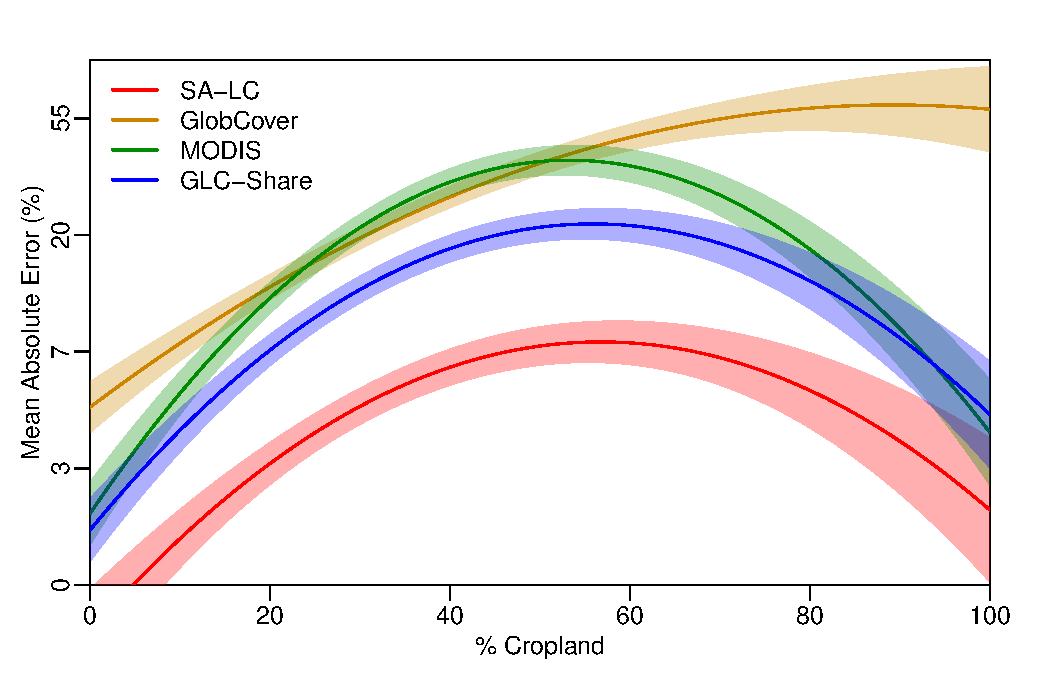
\includegraphics[keepaspectratio,scale = 0.4]{figures/biases_md_lnorm_gam_mu0.pdf}}
\centerline{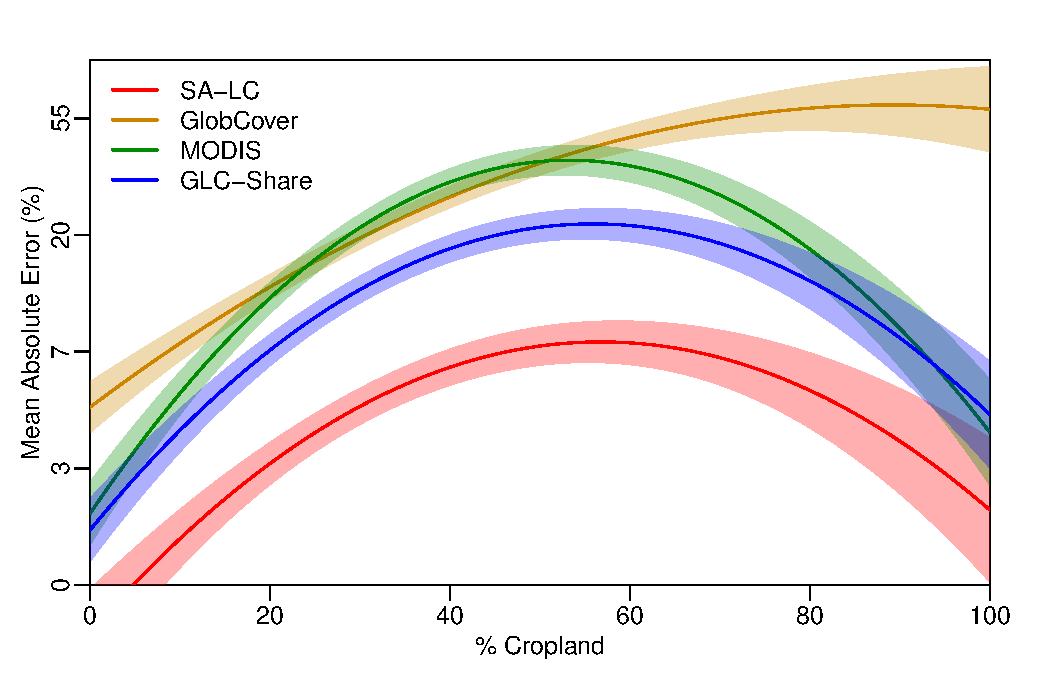
\includegraphics[width=.7\textwidth]{figures/biases_md_lnorm_gam_mu0.pdf}}
\caption{The relationship between map accuracy (the mean absolute error) in test maps and the actual cropland cover within agricultural landscapes (reference map pixels having $>$0.5\% cropland), here defined by the boundaries of magisterial districts (n = 345), as fit with a generalized additive model. Prediction curves are color-coded to the different test maps, with the solid line indicating predicted absolute bias, and the lighter shading the standard error of the coefficients.}\label{afoto2}
\end{figure}
%\end{wrapfigure}
%\vspace{-0.75 cm}


\subsection*{The impact of map error on physical analyses}
\subsubsection*{Carbon estimates}
The spatial patterns of test map errors transmitted into substantial carbon estimation errors, with the sign varying as a function of the density of carbon adjacent to croplands (SI). Where cropland was underestimated and the surrounding cover type was more carbon dense than cropland, carbon density was overestimated, but when the cover type was less dense than croplands (e.g. sparse vegetation), then carbon density was underestimated. The inverse was true where cropland was overestimated. 

The magnitude of carbon errors varied as a function of the carbon density of surrounding cover, as demonstrated by the bias statistics (Fig. 3). Bias was near zero when grassland was the adjacent cover type (SI), as its carbon density is nearly the same as cropland. However, when forest was adjacent then bias was a three- to five-fold multiple of cropland map bias (Fig. 1B). At the most extreme, GlobCover's bias was -276\% at 1 km, but even SA-LC and GeoWiki had biases of 22\% and -50\%, respectively. Bias could be substantial even for the least carbon dense vegetation type (sparse), as evidenced by the 15-25\% mean error at 1 km for MODIS and GlobCover under this class.  The mean bias across the different potential adjacent vegetation classes ranged between -20 for GeoWiki and -123\% for GlobCover at 1 km (with MODIS in between these), while SA-LC's average bias was 11\%.  Biases declined fairly rapidly with aggregation, with all datasets having an average (across cover types) bias magnitude of $<$10\% at $\geq$25 km of aggregation, except for GlobCover, which was -12\% at 100 km (SI).  As with cropland percentages, GeoWiki produced the least biased carbon density estimates above 1 km resolution. 

%\vspace{-0.75 cm}
\begin{figure}[!h]
%\begin{wrapfigure}{r}{0.5\textwidth}
%\centerline{\includegraphics[keepaspectratio,scale = 0.4]{figures/figure3.pdf}}
\centerline{\includegraphics[width=0.55\textwidth]{figures/figure3.pdf}}
\caption{Biases and accuracies (mean absolute errors) of carbon densities derived from cropland maps, calculated as percents relative to the reference map. Bias estimates (represented by symbols) fall within the semi-transparent floating bars, while accuracies are contained in the solid bars. Bar colors are coded to specific cropland map, symbols indicate which cover type was used to calculate cropland-adjacent carbon density. The bar represents the mean biases calculated across each of the 5 cover types. Shrubland and grassland bias values were near zero, while secondary forest values were close to forest values, and thus these are not shown for display clarity (but see Table S2). MODIS and GlobCover values at 1 km exceeding the plot's Y limits are provided near their truncated tops.}
\label{afoto}
\end{figure}
%\end{wrapfigure}

In terms of accuracy, MAE values were essentially the same as bias magnitudes, except for GeoWiki's, which were twice as large. The average MAE across vegetation classes was 47\% at 1 km, dropping to $<$10 only with 25 km of aggregation. In contrast, SA-LC's carbon estimates were twice as accurate at 1 km, and were slightly more accurate up to 25 km of aggregation were GeoWiki achieved parity.  

\subsubsection*{Evapotranspiration estimates}
Compared to the carbon analysis, the bias and accuracy in evapotranspiration (ET) calculated using the VIC model was negligible, averaging less than than +/-2\%. However, there were several error hotspots in the resulting ET residual maps (Fig. 4). The most pronounced of these were the 5-15\% overestimates in the center of the country caused when VIC was initialized with MODIS and GlobCover, while overestimates along the southern and western coasts reached 25\%. These locations correspond primarily to the margins of major crop production regions--in the center is the westernmost boundary of the summer rainfall growing region, marked approximately by the 400 mm isohyet, where maize is the primary crop. The west coast hotspot falls at the western edge of the wheat-dominated winter rainfall region \citep{hardy_rainfed_2011}, where growing season rainfall is approximately 200 mm. 

SA-LC and GeoWiki also resulted in ET errors estimates along the southern and western coasts, but here the tendency was to underestimate ET, while biases in the center of the country were either negligible to absent.  All but MODIS underestimated ET by 5-15\% in the northern tip of the country.  

%\vspace{-0.75 cm}
\begin{figure}[h]
\centerline{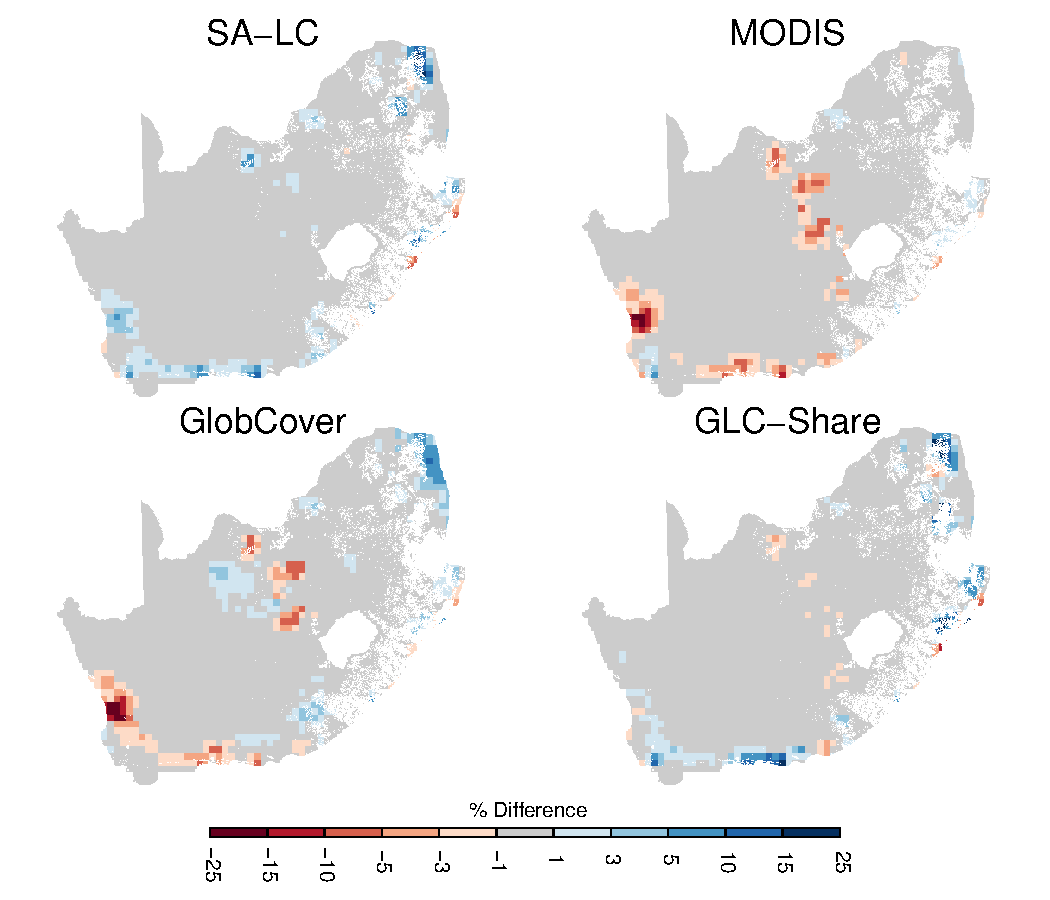
\includegraphics[width=.6\textwidth]{figures/et_bias_map.pdf}}
\caption{Differences in annual mean evapotranspiration estimates from 29-year runs of the VIC land surface hydrology model when initialized with LAI response curves derived from the reference map, versus those from the four test maps.}\label{afoto}
\end{figure}

\subsection*{Socio-economic analyses}
\subsubsection*{Gridded crop yield and production data}
Maize yields disaggregated onto the test maps showed some marked differences relative to the reference map, but only at the margins of the major crop production areas where cropland is sparser (SI). These differences resulted when a yield value was mapped onto a grid cell where the reference map had no harvested area, and thus zero yield. In more densely cropped areas, such discrepancies were less frequent because both the reference and test maps were both likely to have some maize harvested area, and therefore a yield value.  Yield biases were thus fairly low (and accuracy high), with the largest being 20\% for MODIS at 1 km, following by GlobCover with 10\% (Fig. 5). These dropped to $<$10\% with aggregation.  

Production biases were generally slightly higher, but still low, for most datasets, with the exception of GlobCover, which had a large underestimation bias of $>$60\% (relative to mean production) at 1 km, which remained above 10\% even at 100 km of aggregation. MODIS production bias was above 20\% at 1 km, but declined to below 10\% at higher levels of aggregation.  

In contrast, the accuracy of production estimates was poor. Here all datasets but SA-LC had MAE values of $\geq$30\% below 25 km of aggregation (Fig. 5), reaching as high as 100\% for GlobCover at 1 km, followed by 65\% for MODIS and 45\% for GeoWiki. SA-LC estimated production was most accurate, having between 10-20\% MAE between 1 and 10 km, and $<$10\% at 25 km and higher.  This low accuracy relative to the gridded yield measures relates to the disaggregation process for harvested area, which allocates a fractional value to each pixel, which is itself a fraction. The process of adjusting the gridded values so that their totals match reported statistics does relatively little to correct the map's underlying commission or omission errors, and this constraint in fact appears to shorten the distance between negative and positive residuals (SI), thereby increasing absolute errors.  

%\vspace{-0.5 cm}
\begin{figure}[!hb]
%\vspace{-0.75 cm}
\centerline{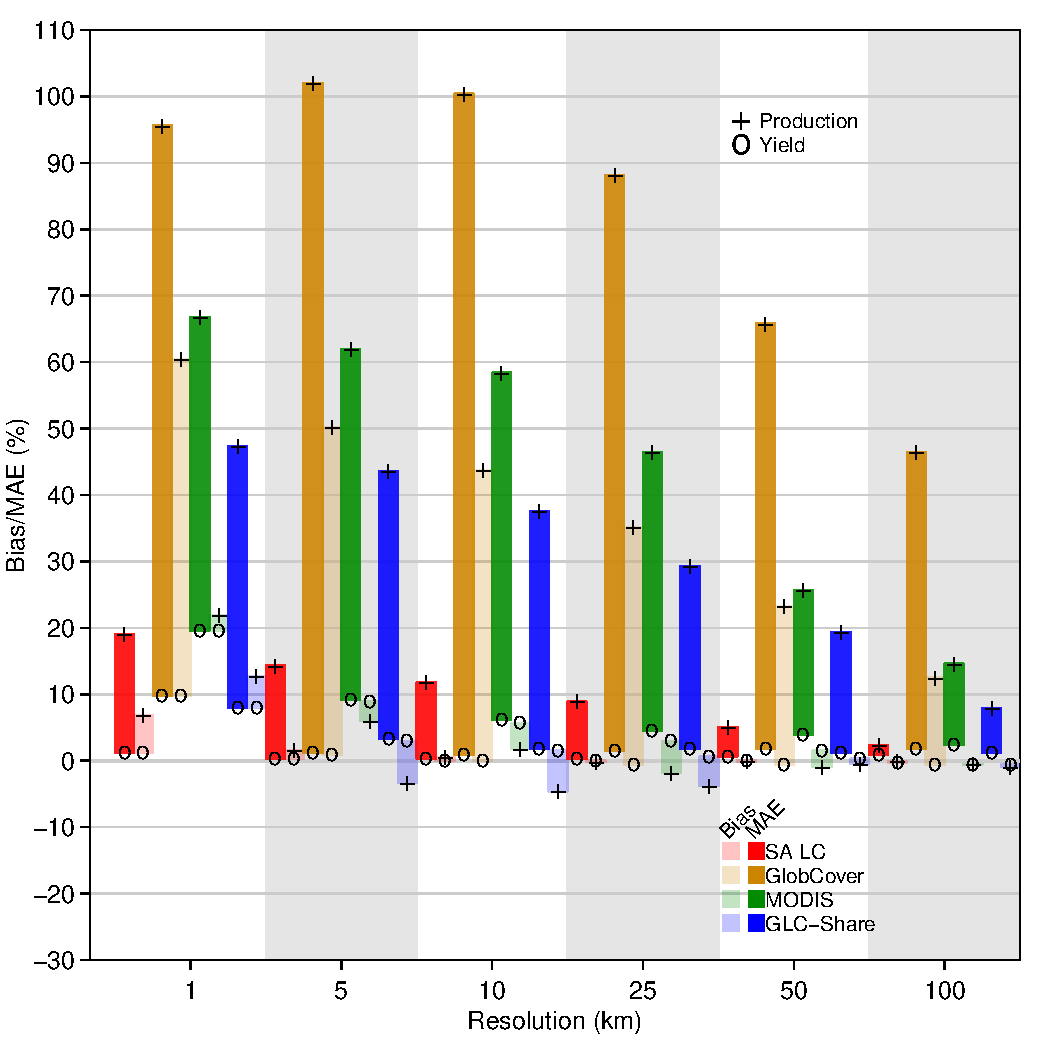
\includegraphics[width=0.55\textwidth]{figures/yield_prod_bias.pdf}}
\caption{Bias (mean error) and accuracy (mean absolute error [MAE]) in disaggregated maize yield and production estimates. Bias estimates (represented by symbols) fall within the semi-transparent bars, mean absolute errors in the solid bars, with bar colors coded to specific cropland maps.  Symbols code the different variables (production and yield), normalized to their respective means.}
\label{afoto}
\end{figure}

\subsubsection*{Agent-based model of household food security}
In terms of impact to agent-based model simulation, where cropland map errors were negative (indicating a cropland overestimate by the test maps), the percent of land left unallocated had a straight one-to-one relationship with the percentage of overestimation (Fig. 6A). When cropland was underestimated, all croplands were allocated up until the underestimation exceeded 50\%. The MODIS-based simulation for districts 1 and 2 was most pronounced for this tendency, with 5-10\% of cropland remaining unallocated despite the fact that the majority of households were not assigned cropland (because cropland was underestimated by 85\%). This non-linear relationship occurred because croplands tend to cluster, and when underestimated clusters tend to be small and isolated, they are more likely to fall outside of the search radius used by the model for allocating fields to households when they are initially seeded onto the landscape. 

Land deficit (the total area of cropland that should have been allocated to households in each district, but wasn't) increased exponentially in relation to cropland underestimation--reaching around 800\% for MODIS in districts 1 and 2 (Fig. 6B)--and would become infinite in the case of a 100\% underestimate. This contrasted with food deficit (the percentage shortfall in the average amount of food production that should have been produced by each household but wasn't), which increased linearly with the percentage of cropland underestimate (Fig. 6C). 

%randomly siting 100 household agents within each district, and allocating the nearest two cropland pixels to each household. The remaining agents are then iteratively assigned unallocated cropland pixels within a 1.5 km radius of existing agents' fields, and this process continues until all agents are assigned cropland, or all available cropland is allocated. This initialization process 
%\FloatBarrier

\begin{figure}[!ht]
\centerline{\includegraphics[width=.55\textwidth]{figures/figure6.pdf}}
\caption{Biases in agent-based model results relative to the district-wise errors (as a percent) in total cropland area, in terms of A) the percent of cropland in each district that was not allocated to any household, B) the land deficit, or the total area of cropland that should have been allocated to households in each district but wasn't (expressed as a percent of total district cropland, as determined by test maps), and C) the food deficit, or the percentage shortfall (relative to the reference simulation) in mean household food production resulting from inadequate cropland allocation. Dot sizes correspond to district numbers, colors represent the landcover map.}
\label{afoto}
\end{figure}

\section*{Discussion}
This spatially comprehensive, bottom-up landcover map assessment provides new insight into the extent and causes of map error, and its consequences for understanding global change. The analysis was made possible by a spatially comprehensive, high accuracy dataset that likely provides the truest measure of cropland area and distribution currently available for this region. Although this reference map is not perfect, being affected by the map-makers' occasional interpretation errors (mostly of omission, SI), while temporal mismatches between the reference and test maps may account for some of the error we identified, our assessment (SI) suggests that such discrepancies do not appreciably impact our findings. Our results are also supported by previous, continental-scale assessments that revealed substantial errors and inconsistencies between landcover maps \citep{fritz_comparison_2010,gross_monitoring_2013}. These similarities, combined with the larger extents of these studies, also suggest that our findings are applicable beyond South Africa's borders.

\subsection*{General guidelines for selecting and using landcover data}
Our findings regarding bias and accuracy suggest several guidelines for selecting and using landcover data in global change research (Table 1), and suggested aggregation scales. These guidelines vary according to the intended application, what error property the users wants to minimize or maximize, and what tradeoff the user is willing to make between error and resolution.  For the purpose of clarity in these guidelines, we assume that a maximum error magnitude of 10\% is acceptable, but the results of our analyses (Fig. 1, 3, 5) allow different thresholds to be  evaluated.  

The first general guideline is that landcover products derived from coarse resolution sensors, such as MODIS and GlobCover, need substantial aggregation to reduce the large biases and inaccuracies that manifest at finer resolutions. Researchers might need to use these datasets for a variety of reasons, for instance, because they provide consistent, multiple landcover classes at a global scale, or allow changes to be tracked across large scales over time \citep{luoto_predicting_2004}. The appropriate scale of aggregation then depends on which error property the user wants to minimize. If the objective is to minimize systematic errors in order to calculate an unbiased mean (e.g. average carbon density), then at least 25-50 km of aggregation is needed to reduce map bias to within +/-10\% (Table 1, Fig. 1B \& 3). If the user wants to maximize accuracy, which is important for comparing differences between locations on a single map, or between dates at fixed locations, then even coarser aggregations are needed to reduce mean absolute error below 10\% (Fig. 1, 3, 5).  

The characteristics of cover at the landscape scale may also require greater levels of aggregation to achieve sufficient accuracy. We found that accuracy is lowest where mixing of cover types is greatest (Fig. 2), a result echoed in an Africa-wide change detection study made with MODIS \citep{gross_monitoring_2013}. Outside of South Africa, where smallholder-driven agriculture predominates \citep{lambin_estimating_2013}, such mixed landscapes are more common, thus greater levels of aggregation may be needed over these areas. Coarser aggregations are also necessary if the cover type of interest belongs primarily to a mixed class (as with GlobCover). This leads to underestimation bias (Fig. 2) and high inaccuracy, which will persist until the aggregated pixel exceeds the characteristic size of the geographical area within which the cover type dominates. In South Africa's farming regions, this can exceed 1000 km$^2$. 

Maps derived from higher resolution sensors, such as the SA-LC dataset, do not have this mixture problem because the pixels are fine enough to be assigned to a single cover type. This characteristic leads to higher accuracy, which is what we observed here: the SA-LC dataset needed the least aggregation--just 5-10 km--to achieve $<$10\% MAE in most of the example applications we tested (note, however, another guideline in this result: even with high resolution maps some aggregation is needed to achieve higher accuracy).

%needed This observation leads to a second rule of thumb: users should select datasets from higher resolution sensors where possible (assuming they were carefully developed), as these needed much less aggregation to return accurate estimates for most applications we tested here. For $<$10\% MAE, just 5-10 km of aggregation were needed (however, this is still much coarser than the 30 m resolution of the sensor itself).    

Unfortunately, Landsat-scaled maps are typically developed for specific countries, using varying methods, and can be hard to obtain (an exception to this is the newly released GLC30, which has a reported classification accuracy of 80\% \citep{chen_global_2015}). Our results also suggest that, despite their higher accuracy, they may not necessarily be the least biased maps. Except for a few results (notably the 1 km carbon and maize production estimates), GeoWiki-based maps had the lowest bias across most scales, which is the largely the result of calibrating the cropland percentages to match reported agricultural statistics \citep{fritz_cropland_2011,fritz_mapping_2015}. This procedure is similar to the one we used in disaggregating maize harvested areas \citep{ramankutty_farming_2008, monfreda_farming_2008}, which led to fairly unbiased estimates of maize production and yield (Fig. 5) above 1 km (except for GlobCover's production estimates). This result, together with GeoWiki's unbiased cropland estimates (Fig 1.B), indicates the value of fusing inventory data with remote sensing to reduce map bias. 

%The consensus method mirrors the ensemble averaging used by other fields (e.g. crop \citep{asseng_uncertainty_2013}, climate \citep{giorgi_calculation_2002}, and ecological modeling \citep{araujo_ensemble_2007}) to increase prediction confidence.

Of course, for the constraint to be effective, the inventory data themselves must be faithful to reality, but in many places, particularly Africa, agricultural statistics are suspect \citep{carletto_emperor_2013, fao_action_2013}, which is a vulnerability of the fusion approach \citep{see_improved_2015}. Beyond this limitation, this method does not improve map accuracy, which is evident in GeoWiki's relatively high MAE for cropland percentage at 1 km (23\%, Fig. 1B), and by all maps' (except SA-LC's) highly inaccurate maize production estimates (Fig. 5). The reason that accuracy is not improved is because the statistical constraint cannot correct the omission and commission errors within the landcover maps. To minimize these types of errors, different techniques are needed, such as creating a single consensus map from multiple landcover products \citep[e.g.][]{fritz_comparison_2010,tuanmu_global_2014}. This second kind of data fusion was used in the first stage of creating the GeoWiki map (before statistical adjustment), and it accounts for GeoWiki's higher accuracy scores relative to MODIS and GlobCover (Fig. 1B, 3, \& 5). It may be particularly effective in minimizing underestimation errors that result when a mixed class type becomes dominant (as with GlobCover), or when dealing with substantial sub-pixel heterogeneity \citep{fritz_mapping_2015,tuanmu_global_2014}

\begin{table*}[!h]
  \begin{threeparttable}
    \caption{Guidelines for selecting and using different classes of landcover product (based on the characteristics of the satellite sensor(s) and map-making methods), according to the general purpose of the application, the error minimization objective, and the range of aggregation needed to achieve the error objective (here we use a maximum acceptable error magnitude of 10\%). The preferred landcover product class for each application is indicated in boldface. }
    \begin{center}
      \begin{tabular*}{\textwidth}{m{3.5cm}m{3cm}m{5.5cm}m{2.25cm}}
       \hline
Application                     & Objective & Source of Landcover Map & Minimum aggregation* \\
\Xhline{1pt}
High frequency            & Maximize accuracy   & Coarse resolution sensor (e.g. MODIS) & $>$100 km\\
change detection                                                               &                                  & \textbf{High resolution sensor} (e.g. Landsat)   &  1-25 km\\
\hline
Mean values         & Minimize bias            & Coarse resolution sensor  & 25-50 km \\
(e.g. carbon density)                                                              &                                   &  \multicolumn{1}{r}{\emph{if mixed class dominates}}                                    & $>$100 km \\
                                                              &                                   & \textbf{Fusion product: statistical constraint} & 1-5 km\\
                                                              &                                   & High resolution sensor & 1-10 km\\
\hline
Spatial comparisons & Maximize accuracy  & Coarse resolution sensor & 25-100 km\\
 (e.g. crop production)                                                               &                                   &  \multicolumn{1}{r}{\emph{if mixed class dominates}}                                    & $>$100 km \\
                                                             &                                   & Fusion product: map consensus** & 10-50 km\\
                                                              &                                   & \textbf{High resolution sensor} & 1-25 km\\
\Xhline{1pt}                         
       \end{tabular*}
       \begin{tablenotes}
        \small
        \item *Aggregation ranges account for variation in the results from the different map analyses.
        \item **This assumes that consensus-based fusion products \citep[e.g.][]{fritz_cropland_2011,fritz_mapping_2015,tuanmu_global_2014} incorporate maps from coarse resolution sensors, making them less accurate at finer scales than products created using high resolution sensors.
       \end{tablenotes}
     \end{center}
     \label{default}
  \end{threeparttable}
\end{table*}


These last few points suggest two final guidelines. For high accuracy, users should select well-validated datasets from higher resolution sensors--this option should be increasingly available as computational power grows and high resolution image archives expand \citep{hansen_high-resolution_2013,chen_global_2015}; 2) where low bias is needed over large areas, the best option is to use newer generation, statistically constrained maps such as GeoWiki (and possibly the GLC-Share \footnote{GLC-Share. www.glcn.org} datasets for other cover types). But in either case some aggregation--1-25 km, depending on application and whether low bias or high accuracy is the objective--will still likely be necessary to achieve sufficiently low error. Additionally, these higher accuracy, lower bias products often represent just a single time period \citep[e.g.][]{fritz_mapping_2015,tuanmu_global_2014}, thus applications requiring higher frequency (e.g. annual), large area landcover maps will depend on MODIS or similar sensors, and therefore much coarser aggregations.  

%GeoWiki was the most accurate among the large scale landcover products, but its improvement is related to the map consensus methods, which can correct for omission or commission errors made by the classifier. 

\subsection*{Implications for global change analyses}
Besides the preceding landcover data selection and usage guidelines, our findings also have broader implications for global change analyses and associated policy decisions. The simpler, most direct uses of landcover data have substantial potential to skew our understanding of global change processes. For example, the global carbon carbon density map of \citep{ruesch_new_2008}, of which we created facsimiles here, has been widely used, but our results suggest that any analyses of the spatial variability of carbon stocks, or of mean carbon densities, can be highly misleading if the map is not first sufficiently aggregated. For example, a study of deforestation risks in the Democratic Republic of the Congo estimated forest rents as a function of carbon densities based on this map. Although the map was aggregated to $\sim$50 km, we found that mean absolute errors can still reach 40\% at this scale (Fig. 3). The same carbon map provided country-specific mean forest carbon densities for an evaluation of climate mitigation policies \citep{cattaneo_international_2010}, which our results suggest could be substantially underestimated (Fig. 3). In contrast to these, an assessment of the congruence between carbon and biodiversity \citep{strassburg_global_2010} aggregated the carbon densities to $\sim$110 km, where accuracy is much higher. 

A related example can be seen in high resolution maps (10 km) showing the potential food production benefit of closing yield gaps \citep[e.g. Figure 3 in][]{foley_solutions_2011}. Such maps may give an inflated sense of the precision with which such locations can be identified. Although the study in this example is careful to report aggregated statistics and maps the per hectare values, and the map-makers stress that their products should not be used at the grid cell scale\footnote{www.earthstat.org\/wp-content\/uploads\/METADATA\_HarvestedAreaYield175Crops.pdf}, it is not inconceivable that users might make decisions based on their visual interpretations of maps. For this reason, it is advisable to aggregate presented maps until their accuracy reaches an acceptable standard (Table 1). 

What then, of the impacts of landcover map error on more complex analysis?  Here the results appear to be mixed. Map error appears to have had little impact on the overall bias and accuracy of VIC's evapotranspiration (ET) estimates, which contrasts with a related study that examined how landcover maps impact rainfall simulations \citep{ge_impacts_2007}. There are two reasons for this. First, map accuracy increased nearly two-fold by aggregating to 25 km, the resolution of VIC. Second, VIC's landcover-derived variables (e.g. LAI curves, effective rooting depth) could dampen the effect of map errors on ET calculations when the values of these variables in the adjacent landcovers are similar to that of cropland, which is the case in much of VIC's landcover scheme for South Africa. In other regions, where the matrix landcover's LAI values depart substantially from cropland's (e.g. in forest), the ET errors would likely be much larger. The carbon example illustrates how cover properties can mute or amplify map error.  

Despite the low values of the overall error metrics, the hotspots of ET errors (Fig. 4) may have outsize significance because they occurred at the climatic margins of the major crop growing regions, where a substantial share of farms are irrigated. Since VIC does not simulate irrigation, the magnitude of these errors is likely to have been underestimated, because irrigation substantially increases latent heat flux and can substantially modify regional climate \citep{sacks_effects_2008,mueller_cooling_2015}. This also suggests the potential for map error to magnify in a coupled land-atmosphere model \citep[which could explain the difference between this result and that of][]{ge_impacts_2007}, and thereby give misleading insight into the climatic effects of land use.     

Relative to the ET example, map errors had a much larger impact on the agent-based model's results. For the model's most important metric of food security--household-level crop production--the result was fairly straightforward for a class of models where the interactions of multiple agents often produce analytically intractable outcomes \citep{janssen_empirically_2006}. In this case, the model was only sensitive to cropland underestimates, which had the perfectly predictable effect of lowering average household food production, which would in turn overstate the degree of food \emph{in}security. Overestimates did not matter in this case, because the number of households remained fixed, and their cropland holdings were constrained to match the survey statistics (but this would matter for models that allow these parameters to vary). Less predictable was the finding that the spatial distribution of cover can impact model parameterization, with land being left unallocated even when needed, thus such models also require spatial, not just statistical, accuracy in their base landcover maps.  

The errors in the cropland data we tested were large, and it is unlikely that current ABM-based studies, mostly of small regions, are based on such inaccurate landcover data. However, as computing power increases, so, too, does the feasible application extent of ABMs, which will then become more reliant on larger-scaled, more erroneous, landcover data, with the attendant risk that insights into socio-ecological systems arising from these models could be highly misleading.  

Beyond these examples, there are other applications where landcover map errors could alter understanding and policy. One of these lies in assessments of land availability for agricultural expansion, which could be particularly erroneous if they use a ``residual approach'' \citep{lambin_estimating_2013}, where existing cropland and other occupied cover types are used to filter a map of potential suitability. Our results suggest that the pronounced underestimation biases (Fig. 1) we found could inflate land availability estimates, and therefore increase the risk of unjust land allocation policies \citep{rulli_global_2013}. Another example is the growing efforts to minimize the environmental and climate impacts on new agricultural expansion frontiers, particularly Africa's savannas, which requires identifying areas that provide the highest agricultural benefit for the lowest environmental cost \citep{searchinger_high_2015}. This sort of analysis entails finding ``win-win'' land use solutions, which are essentially areas that deviate from an expected development cost-benefit relationship; for example, regions of unusually low carbon density but high crop fertility \citep{searchinger_high_2015}. The validity of such analysis are entirely dependent In order to be effective, such analyses must be undertaken at the fine scales--hectares, rather than square kilometers--at which land use decisions are made, thus their value for informing land use policy is contingent on the accuracy of their underlying landcover/land use data \citep{searchinger_high_2015}. The validity of such analyses, which must be undertaken at the fine-scales where land use decisions are made (hectares rather than square kilometers), depends on having high quality map data, in order to have confidence that the identified tradeoffs are based on real biophysical properties, not simply map error.

\subsection*{The way forward}
Our analysis demonstrates that the landcover data that increasingly inform much global change research and policy can be substantially misleading, depending on the dataset selected, its application case, the scale to which it is aggregated, and whether the insight being drawn from the map depends on how accuracy or low bias. We provide some basic guidelines (Table 1) for selecting and using landcover data that can help increase confidence in the conclusions drawn from landcover-based studies. 

Beyond these guidelines, we recommend updating several important, global-scale datasets using the latest generation landcover maps. For example, rebuilding the widely used cropland distribution and yield maps \citep{monfreda_farming_2008, ramankutty_farming_2008} using the GeoWiki map could substantially improve our knowledge about current global agricultural distribution and productivity. Similarly, reconstructing the IPCC's Tier 1 vegetative carbon map \citep{ruesch_new_2008} using a combination of the GeoWiki and new global landcover consensus maps \citep[e.g. GLC-Share or][]{tuanmu_global_2014} the GLC-Share datasets would improve our confidence in regional to global assessments of vegetative carbon stocks. Alternatively, the new high-resolution, Landsat-based GLC30 \citep{chen_global_2015}, aggregated and converted to fractional cover classes at 1 km--and fused with high quality national landcover maps, where available \citep[similar to][]{fritz_mapping_2015,fritz_cropland_2011}--may provide a preferable base map for rebuilding these datasets. 

Fusing human judgement with expanding high resolution satellite data archives, improved classification algorithms, and expanding computing power appears to offer the greatest promise for improving the quality of landcover maps. The GeoWiki project and new high resolution global forest change maps \citep{hansen_high-resolution_2013,sexton_conservation_2015} are prominent examples of these newer methods. Another approach is that of the Mapping Africa project\footnote{http://mappingafrica.princeton.edu}, which, inspired by quality of the reference map used in this study, enlists internet-based workers to manually digitize cropland boundaries \citep{estes_platform_2016}. Merging this crowdsourced approach for creating vector maps of discrete cover types with newer computer vision-based mapping algorithms \citep{debats_generalized_2016} is a near-term goal of this project, as the former can interactively provide high quality training and test data (by using humans' superior capacity to delineate discrete cover types in noisy images \citep{estes_platform_2016}) for the latter, which has the advantage of speed and the ability to handle high-dimensional datasets. Approaches such as these will be needed to create the next generation of landcover maps, so that we can gain a clearer, unbiased understanding of global change. 

% $\theta$ changes from 0 to 1. (see Figure \ref{afoto}).That means we are considering $\theta$  of the form
%For these solutions we have the following

%\begin{remark}
%Note that equation \eqref{theta} specifies  the function $\varphi$
%up to an error of order $\delta$. Theorem 1 provides an evolution
%equation for the function $\varphi$ up to an error of order
%$\delta |log \delta|$.
%\end{remark}

%(see \eqref{weaksol}). 


%\begin{materials}

%\end{materials}

%\appendix[App 1]

%\appendix
%This is an example of an appendix without a title.

\section*{Acknowledgments}
This work was supported by funds from the Princeton Environmental Institute Grand Challenges program, the NASA New Investigator Program (NNX15AC64G), and the National Science Foundation (SES-1360463 and BCS-1026776). We thank Tobias Kuemmerle for his helpful review of our study and suggestions for improvement. 
%\end{acknowledgments}


\bibliographystyle{gcbnourl} 
{\footnotesize \bibliography{/Users/lestes/Dropbox/publications/full.bib}}

%\end{article}

%\begin{figure}
%\centerline{\includegraphics[width=.4\textwidth]{figsamp.eps}}
%\caption{LKB1 phosphorylates Thr-172 of AMPK$\alpha$ \textit{in vitro}
%and activates its kinase activity.}\label{afoto}
%\end{figure}
%
%\begin{figure*}[ht]
%\begin{center}
%\centerline{\includegraphics[width=.7\textwidth]{figsamp.eps}}
%\caption{LKB1 phosphorylates Thr-172 of AMPK$\alpha$ \textit{in vitro}
%and activates its kinase activity.}\label{afoto2}
%\end{center}
%\end{figure*}
%
%\begin{table}[h]
%\caption{Repeat length of longer allele by age of onset class.
%This is what happens when the text continues.}
%\begin{tabular}{@{\vrule height 10.5pt depth4pt  width0pt}lrcccc}
%&\multicolumn5c{Repeat length}\\
%\noalign{\vskip-11pt}
%Age of onset,\\
%\cline{2-6}
%\vrule depth 6pt width 0pt years&\multicolumn1c{\it n}&Mean&SD&Range&Median\\
%\hline
%Juvenile, 2$-$20&40&60.15& 9.32&43$-$86&60\\
%Typical, 21$-$50&377&45.72&2.97&40$-$58&45\\
%Late, $>$50&26&41.85&1.56&40$-$45&42\tablenote{The no. of wells for all samples was 384. Genotypes were
%determined by mass spectrometric assay. The $m_t$ value indicates the
%average number of wells positive for the over represented allele.}
%\\
%\hline
%\end{tabular}
%\end{table}
%
%
%\begin{table*}[ht]
%\caption{Summary of the experimental results}
%\begin{tabular*}{\hsize}
%{@{\extracolsep{\fill}}rrrrrrrrrrrrr}
%\multicolumn{3}{l}{Parameters}&
%\multicolumn{5}{c}{Averaged Results}&
%\multicolumn{5}{c}{Comparisons}\cr
%\hline
%\multicolumn1c{$n$}&\multicolumn1c{$S^*_{MAX}$}&
%\multicolumn1c{$t_1$}&\multicolumn1c{\ $r_1$}&
%\multicolumn1c{\ $m_1$}&\multicolumn1c{$t_2$}&
%\multicolumn1c{$r_2$}&\multicolumn1c{$m_2$}
%&\multicolumn1c{$t_{lb}$}&\multicolumn1c{\ \ $t_1/t_2$}&
%$r_1/r_2$&$m_1/m_2$&
%$t_1/t_{lb}$\cr
%\hline
%10\tablenote{Stanford Synchrotron Radiation Laboratory (Stanford University,
%Stanford, CA)}&1\quad &4&.0007&4&4&.0020&4&4&1.000&.333&1.000&1.000\cr
%10\tablenote{$R_{\rm FREE}=R$ factor for the $\sim 5$\% of the randomly
%chosen unique ref\/lections not used in the ref\/inement.}&5\quad &50&.0008&8&50&.0020&12&49&.999&.417&.698&1.020\cr
%100\tablenote{Calculated for all observed data}&20\quad &2840975&.0423&95&2871117&.1083&521&---&
%.990&.390&.182&---\ \ \cr
%\hline
%\end{tabular*}
%\end{table*}


\end{document}


